\documentclass[addpoints]{exam}

% \pagestyle{empty}                       %no page numbers
% \thispagestyle{empty}                   %removes first page number
% \setlength{\parindent}{0in}               %no paragraph indents

\usepackage{fullpage}
\usepackage[tmargin = 0.5in, bmargin = 1in, hmargin = 1in]{geometry}     %1-inch margins
\geometry{letterpaper}                  
\usepackage{graphicx}
\usepackage{amssymb}

% Default packages
\usepackage{latexsym}
\usepackage{amsfonts}
\usepackage{amsmath}
\usepackage{amsthm}
\usepackage{palatino}
\usepackage{hyperref}
\usepackage{multicol}
\usepackage{multirow}
\usepackage{enumerate}
\usepackage{enumitem}


%% Definitions
\def\vi{\mathbf{i}}
\def\vj{\mathbf{j}}
\def\vk{\mathbf{k}}
\def\vr{\mathbf{r}}
\def\vu{\mathbf{u}}
\def\vv{\mathbf{v}}
\def\pageturn{\vfill
\begin{flushright}
	\begin{small}
		Continued $\rightarrow$
	\end{small}
\end{flushright}
\newpage}

\pagestyle{headandfoot}
\runningheadrule
\firstpageheader{\textbf{MTH 210 (Talbert)}}{\textbf{Section 02 FINAL EXAM Solutions \ points}}{\textbf{December 12, 2012}}
\runningheader{MTH 210}
{MTH 210 FINAL EXAM, Page \thepage\ of \numpages}
{Dec 12, 2012}
\firstpagefooter{}{}{}
\runningfooter{}{}{}

\printanswers


\begin{document}

		
\vspace*{0pt}

\noindent
Name: \underline{\hspace{2in}} \\


\noindent
\textbf{Instructions}: Welcome to your Final Exam. You may use three $3 \times 5$ notecards with notes and a calculator. You may NOT use any device that can communicate  with another device. The backs of each page are blank; use them if needed. On all questions other than multiple choice, give complete and correct solutions; answers without accompanying work will be given no credit. 

The test will end promptly at 12:00pm. No extensions or extra time will be given unless you have received prior permission from the instructor.

\begin{questions}

	
\uplevel{\emph{Items 1---12 are multiple choice questions that address a variety of learning objectives. Please circle the ONE response you believe is most correct. You do not need to justify your answer.}}

\question[2] Which of the following are statements? 
\begin{parts}
	\part $3^2 + 4^2 = 5^2$. 
	\part Prove or disprove that $3^2 + 4^2 = 5^2$. 
	\part $3^2 + 4^2 \neq 5^2$. 
	\part All of the above
	\part Just (a) and (c)
\end{parts}

\begin{solution}
	\textbf{E}. Both of those sentences are declarative sentences with a definite true/false value. Option B is not a declarative sentence. 
\end{solution}


\question[2] Suppose you wanted to prove that the following statement is FALSE: ``There exists a bijection $f: \mathbb{N} \to \mathbb{Z}$''. An appropriate technique for doing so would be
	\begin{parts}
		\part To give an example of a function $f: \mathbb{N} \to \mathbb{Z}$ that is a bijection
		\part To give an example of a function $f: \mathbb{N} \to \mathbb{Z}$ that is not a bijection
		\part To give a formal proof that all functions $f: \mathbb{N} \to \mathbb{Z}$ are bijections
		\part To give a formal proof that all functions $f: \mathbb{N} \to \mathbb{Z}$ fail to be bijections
		\part None of the above
	\end{parts}

	\begin{solution}
		\textbf{D}. Proving the original statement false amounts to proving its negation is true, which is that every function $f: \mathbb{N} \to \mathbb{Z}$ is not a bijection. 
	\end{solution}

\question[2] The negation of the statement ``If $A$, then $B$'' is
		\begin{parts}
			\part If $A$, then not $B$. 
			\part If not $A$, then $B$.
			\part Not $A$ and not $B$. 
			\part Not $A$ or not $B$. 
			\part None of the above
		\end{parts}

		\begin{solution}
			\textbf{E}. The correct negation is ``$A$ and not $B$''.
		\end{solution}



% \question[2] Consider the conditional statement: ``If $f$ is differentiable at $x=a$, then $f$ is continuous at $x=a$.'' Which of the following statements is logically equivalent to this statement? 
% 				\begin{parts}
% 					\part If $f$ is continuous at $x=a$, then $f$ is differentiable $x=a$. 
% 					\part If $f$ is not differentiable at $x=a$, then $f$ is not continuous at $x=a$ 
% 					\part If $f$ is not continuous at $x=a$, then $f$ is not differentiable at $x=a$. 
% 					\part All of the above
% 					\part Just (c) and (d)
% 				\end{parts}

\question[2] Under what conditions will the conditional statement $A \rightarrow (B \vee C)$ be true? 
	\begin{parts}
		\part When $A$ is true and $C$ is false
		\part When $A$ is false
		\part When $B$ is false
		\part All of the above
		\part Just (b) and (c)
	\end{parts}

\begin{solution}
\textbf{B.} If the hypothesis is false, the entire conditional statement is true. In (a), the statement is definitely FALSE. In (c), the statement might be true or it might be false -- not enough information to say. 
\end{solution}

\question[2] Consider the statement: ``For all integers $k$, $k^2 + 2k - 1$ is not a multiple of $4$.''. A mathematically correct strategy for proving this statement would be
	\begin{parts}
		\part Give an example of an integer $k$ such that $k^2 + 2k - 1$ is not a multiple of $4$. 
		\part Give an example of an integer $k$ such that $k^2 + 2k - 1$ \emph{is}  a multiple of $4$. 
		\part Assume $4$ divides $k^2 + 2k - 1$ and then provide an example of where this fails, thereby arriving at a contradiction. 
		\part Assume $4$ divides $k^2 + 2k - 1$ for some integer $k$ and then arrive at a contradiction. 
		\part Both (c) and (d)
	\end{parts}

	\begin{solution}
		\textbf{D}. 
	\end{solution}

% \question[2] 	What is the main difference between the Extended Principle of Mathematical Induction and the ``basic'' Principle of Mathematical Induction? 
% 	\begin{parts}
% 		\item The Extended Principle allows you to use induction on real numbers, not just natural numbers
% 		\item The Extended Principle allows you to start at a different base case 
% 		\item The Extended Principle changes the inductive hypothesis to assume the truth of each statement $P(1), P(2), \dots, P(k)$ for some $k \in \mathbb{N}$
% 		\item The Extended Principle has more words in it
% 	\end{parts}

\question[2] Suppose that $f$ and $g$ are two equal functions, the domain of $g$ is $\mathbb{Z}$, and that $g(-2) = 3$. Then based on this information alone, we can conclude that 
	\begin{parts}
		\item The domain of $f$ is $\mathbb{Z}$
		\item The codomain of $f$ is $\mathbb{Z}$
		\item $f(-2) = 3$
		\item All of the above
		\item Just (a) and (c)
	\end{parts}

	\begin{solution}
		\textbf{E.} The domains of $f$ and $g$ must be equal and $f(x) = g(x)$ for all $x$ in the domain. We do not know what the codomain of $g$ is, so we can't say what the codomain of $f$ is. 
	\end{solution}


% \question[2] To prove that three separate statements $A$, $B$, and $C$ are equivalent, we need to show
% \begin{parts}
% 	\item $A$ implies $B$
% 	\item $B$ implies $C$
% 	\item $C$ implies $A$
% 	\item All of the above
% 	\item Just (a) and (b)
% \end{parts}


\question[2] Which of the following functions $f: \mathbb{Z} \to \mathbb{Z}$ is a surjection? 
	\begin{parts}
		\part $f(a) = a^2$ 
		\part $f(a) = a^3$
		\part $f(a) = a \pmod {10}$
		\part All of the above
		\part None of the above
	\end{parts}

	\begin{solution}
		\textbf{E}. The function in (a) is not a surjection because there is no $x \in \mathbb{Z}$ such that $f(x) = -1$. The function in (b) is not a surjection because there is no $x \in \mathbb{Z}$ such that $f(x) = 2$. The function in (c) is not a surjection because there is no $x \in \mathbb{Z}$ such that $f(x) = 11$. 
	\end{solution}


\question[2] Suppose $f: \mathbb{R} \rightarrow \mathbb{R}$ is given by $f(x) = 3 + 2^x + 4x$. This function is a bijection. The value of $f^{-1}(4)$ is 
	\begin{parts}
		\part $-4$
		\part $0$
		\part $1/35$
		\part $1/4$
		\part $35$
	\end{parts}

\begin{solution}
	\textbf{B}. This is because $f(0) = 4$. 
\end{solution}


\question[2] Let $\sim$ be the relation on $\mathbb{R}$ given by $x \sim y$ if and only if $x-y$ is divisible by $5$. Then $\sim$ is 
	\begin{parts}
		\part Reflexive
		\part Symmetric
		\part Transitive
		\part All of the above
		\part Just (a) and (b) 
	\end{parts}

\begin{solution}
	\textbf{D}. This relation is actually the same as integer congruence mod 5, which we have seen and proven satisfies all three of reflexivity, symmetry, and transitivity. 
\end{solution}


\question[2] Let $\sim$ be an equivalence relation on a nonempty set $A$ and suppose $a, b \in A$. Then $[a] = [b]$
	\begin{parts}
		\part Always
		\part Only if $a = b$
		\part Only if $a \sim b$
		\part Only if $[a]$ and $[b]$ are disjoint
		\part Never
	\end{parts}

	\begin{solution}
		\textbf{C}. This is Theorem 7.14(b), one of the major results of Chapter 7. 
	\end{solution}

\question[2] To prove that a function $f: A \to B$  is a surjection,
	\begin{parts}
		\part Let $a \in A$ and prove that $f(a)$ is a unique point in $B$. 
		\part Let $a, a' \in A$ with $a \neq a'$, and prove that $f(a) \neq  f(a')$. 
		\part Let $a, a' \in A$ with $f(a) \neq f(a')$, and prove $a \neq a'$.  
		\part Let $b \in B$, and prove there exists $a \in A$ such that $f(a) = b$. 
		\part Both (b) and (c)
	\end{parts}
	
\begin{solution}
	\textbf{D}. This is the definition of surjection. 
\end{solution}

\question[2] To show that a function $f: A \to B$  is \emph{not} an injection,
	\begin{parts}
		\part Show that there exists a point $a \in A$ such that $f(a)$ maps to two different points in $B$. 
		\part Show that there exists two points $a, a' \in A$ such that $f(a) \neq f(a')$.
		\part Show that there exists two points $a, a' \in A$ such that $a \neq a'$ but $f(a) = f(a')$. 
		\part Either (b) or (c)
		\part None of the above
	\end{parts}

\begin{solution}
	\textbf{C}. This is the definition of injection. You need the two points to be different in order to satisfy that definition, hence choice (b) is not correct. 
\end{solution}



%%% COMPUTATION

\question Below are a variety of computations to carry out. Do each one. You do not need to show work, but if you make a mistake, partial credit will be awarded only if there is supporting work. 
	\begin{parts}
		\part[6] Let $f: \mathbb{Z} \to \mathbb{Z}$ be defined by $f(a) = a^2 \pmod {11}$. Fill in the following table: 


			\begin{solution}

				\begin{center}
				\begin{tabular}{c||c|c|c|c|c}
				$a$ & $-4$ & $-2$ & $0$ & $2$ & $4$ \\ \hline
				$f(a)$&  5 & 4 & 0 & 4 & 5
				\end{tabular}
			\end{center}

			\end{solution}




		
		\part[6] Let $A = \{ 1, 2,3 , 4\}$, $B = \{ 3, 4, 5, 6\}$, and $C = \{ 6, 7\}$ Calculate the set $A \times (C - B)$. 
		
\begin{solution}
	We have $C - B = \{ 7 \}$. This gives: 
	\[ A \times (C-B) = \{ 1,2,3,4 \} \times \{ 7 \} = \{ (1, 7), (2, 7), (3, 7), (4, 7) \} \]
\end{solution}

		
		\part[6] Find the integers $q$ and $r$ guaranteed by the Division Algorithm such that $1192009 = 6q + r$. 
		
\begin{solution}
	Long division shows that $6$ divides $1192009$, $198668$ times with a remainder of $1$. Therefore $q = 198668$ and $r=1$. 
\end{solution}

		
		\part[6] Let $\sim$ be the relation on $\mathbb{Z}$ defined as follows: For all $a,b \in \mathbb{Z}$, $a \sim b$ if and only if $a-b$ is a multiple of 3. It can be proven that $\sim$ is an equivalence relation. Write the elements of $[1492]$ as a set in roster form. 

		\begin{solution}
			The set $[1492]$ is the set of all integers $n$ such that $1492 - n$ is a multiple of 3 --- in other words, it's the set of all integers that are congruent to 1492 mod 3. Since $1492 \pmod 3 = 1$, we have
			\[ [1492] = \{\dots, -8, -5, -2, 1, 4, 7, 10, 13, \dots, 1399, 1492, 1495, \dots \}\]
		\end{solution}

		
		\part[6] Let $\sim$ be the relation on the set $A = \{1, 2, 3, \dots, 10\}$ defined by $a \sim b$ if and only if $a$ divides $b$. Draw the directed graph for this relation. 
	\end{parts}

		\begin{solution}
			Here's the directed graph: 
			\begin{center}
				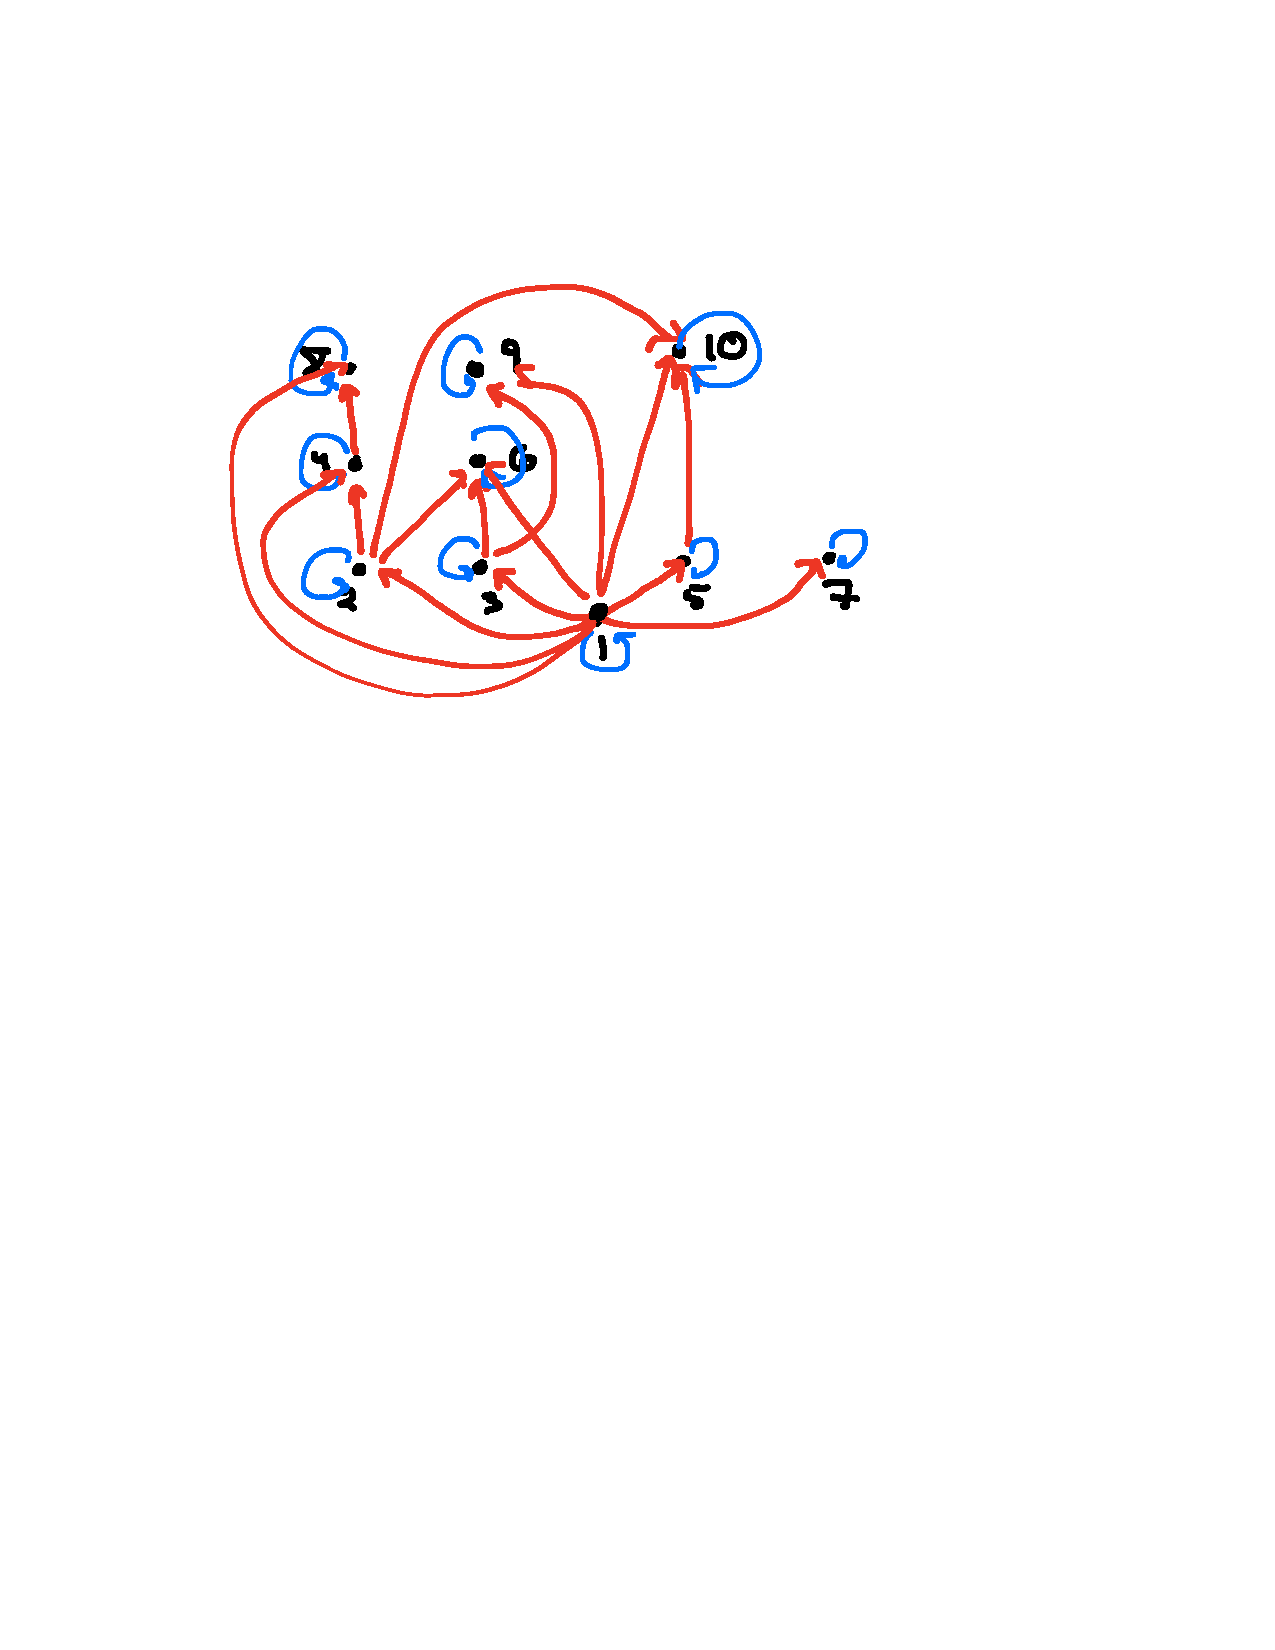
\includegraphics[width=2in]{digraph}
			\end{center}
			
	Key features: there is an arrow from 1 to everything else; every vertex has a loop; and whenever $a$ divides $b$ there is an arrow from $a$ to $b$. 
		\end{solution}


	
\question For each of the following statements, write the negation of the statement in symbolic form in which the negation symbol ($\neg$) is not used, and then write the negation as an English sentence. 
	\begin{parts}
		\part[6] $(\exists x \in \mathbb{R})(\cos(2x) = 2 \cos x)$
		
		\begin{solution}
			\[ (\forall x \in \mathbb{R})(\cos(2x) \neq 2 \cos x) \]
			For every real number $x$, $\cos(2x)$ does not equal $2 \cos x$. 
		\end{solution}		
		
		\part[6] $(\forall x \in \mathbb{Z})((2|x) \Rightarrow (4|x))$ (The arrow ($\Rightarrow$) means ``implies''.) 
		
		\begin{solution}
			\[ (\exists x \in  \mathbb{Z})((2 | x) \wedge (4 \not | x)) \]
			There exists an integer $x$ such that $2$ divides $x$ but $4$ does not divide $x$.

		\end{solution}
		
	\end{parts}
	
	

\question Consider the statement: 		\emph{If it is snowing and after 6:00am, then I will shovel my driveway.}

	\begin{parts}
		\part[6] Write a clear statement of the contrapositive of this sentence. 
		
		\begin{solution}
			If I did not shovel my driveway, then either it is not snowing or it is not after 6:00am. 
		\end{solution}
		
		\part[6] Write a clear statement of the converse of this sentence. 
		
		\begin{solution}
			If either it is not snowing or it is not after 6:00am, then I did not shovel my driveway.
		\end{solution}
		
	\end{parts}


\pageturn

% \uplevel{\emph{The next several items are problems to solve. Each item is tagged with a list of learning objectives it assesses. Be sure to give complete, clear, and correct solutions to each, not just answers.}}
% 	


% At least 1 of the following should be done on a setup level only.


\question Below are several proof-related tasks that we have undertaken repeatedly during the course. For each task, give a brief but complete outline of how a correct proof would be constructed in that situation. Be sure to state explicitly \textbf{what you would assume,  what you would try to prove, and a  specific strategy for how you would proceed from the beginning}. 
	\begin{parts}
		\part[8] Proving that two sets, $A$ and $B$, are equal via the ``choose an element'' approach

		\begin{solution}
			We would need to show that $A \subseteq B$ and $B \subseteq A$. For the first part, choose an element $x \in A$ and then prove that $x \in B$. For the second, choose an element $y \in B$ and prove that $y \in A$. 
		\end{solution}
				
		\part[8] Proving the conditional statement ``If $P$, then $Q$'' by contraposition
		
\begin{solution}
	We first form the contrapositive of the statement, which would say ``If $\neg Q$, then $\neg P$.'' Then assume $\neg Q$. End by proving (through valid mathematical steps) the truth of $\neg P$. 
\end{solution}
		
		
		
		
		\part[8] Proving that the predicate $P(n)$ is true for all natural numbers $n$ using mathematical induction
		
		\begin{solution}
			We first prove that $P(1)$ is true, thereby establishing that there is some case in which the predicate is true. Then we assume that $P(k)$ is true for some natural number $k$, and then use this assumption along with valid mathematical steps to prove that $P(k+1)$ is true. 
		\end{solution}
		
	\end{parts}


\question[16] Choose EXACTLY ONE of the following and either prove the statement or disprove it. Circle the letter of the problem you are doing. 
	\begin{parts}
		\part For all integers $a,b$ and $d$ with $d \neq 0$, if $d$ divides $a$ or $d$ divides $b$, then $d$ divides $ab$. 
		
			\begin{solution}
				This statement is true. Here is a proof. \\

				Assume that either $d$ divides $a$ or $d$ divides $b$. We will show that $d$ divides $ab$. We will use two cases, depending on which integer $d$ divides. 
				\begin{description}
					\item[Case 1: $d|a$.] Suppose $d|a$. This means there is an integer $q$ such that $a = dq$. Multiplying both sides of this equation by $b$, we have $ab = d(bq)$. Since $q$ and $b$ are integers, so is $bq$ by closure; therefore we see that $d$ divides $ab$. 
					\item[Case 2: $d|b$.] Suppose $d|b$. This means there is an integer $q$ such that $b = dq$. Multiplying both sides of this equation by $a$, we have $ab = d(aq)$. Since $q$ and $a$ are integers, so is $aq$ by closure; therefore we see that $d$ divides $ab$. 
				\end{description}
		In either case, $d$ divides $ab$ as desired. 	
			\end{solution}
		
		\part For all functions $f: A \to B$ and $g: B \to C$, if $g \circ f: A \to C$ is an injection then  $f$ is an injection. 
		
		\begin{solution}
			The statement is true. Here is a proof. \\

			We will prove the contrapositive. So suppose that $f$ is not an injection; we will show that $g \circ f$ is not an injection. Since $f$ is not an injection, then there exist points $x_1, x_2 \in A$ such that $x_1 \neq x_2$ but $f(x_1) = f(x_2)$. But then since $f(x_1) = f(x_2)$, we have $g(f(x_1)) = g(f(x_2))$. This means that $x_1 \neq x_2$ but $(g \circ f)(x_1) = (g \circ f)(x_2)$. Hence $g \circ f$ is not an injection, and we are done. 

		\end{solution}
		
		\part For each integer $n$, if $n$ is odd, then $8$ divides $n^2 - 1$. 
		
		\begin{solution}
			The statement is true. Here is a proof. \\

			Suppose that $n$ is odd. We will show that $8$ divides $n^2 - 1$. Since $n$ is odd, there is an integer $q$ such that $n = 2q + 1$. Now compute $n^2 - 1$: 
			\begin{align*}
				n^2 - 1 &= (2q+1)^2 - 1 \\
						&= 4q^2 + 4q + 1 - 1 \\
						&= 4q^2 + 4q
			\end{align*}
			Now we can proceed by two cases: One if $q$ is even and another if $q$ is odd. 
			\begin{description}
				\item[Case 1: $q$ is even.] Suppose $q = 2k$ for some integer $k$. Then going back to $n^2 - 1$, we have: 
				\[ n^2 - 1 = 4q^2 + 4q = 4(2k)^2 + 4(2k) = 16k^2 + 8k = 8(2k^2 + k) \]
				Since $k$ is an integer, so is $2k^2 + k$ by closure. Thus we see that in this case, $8$ divides $n^2 - 1$. 
				\item[Case 2: $q$ is odd.] Suppose $q = 2l+1$ for some integer $l$. Then going back to $n^2 - 1$, we have: 
				\[ n^2 - 1 = 4q^2 + 4q = 4(2l+1)^2 + 4(2l+1) = 16l^2 + 24l + 8 = 8(2l^2 + 3l + 1) \]
				Since $l$ is an integer, so is $2l^2 + 3l + 1$ by closure. Thus we see that in this case, $8$ divides $n^2 - 1$.
			\end{description}
			In either case, we proved what we set out to prove, namely that $8$ divides $n^2 - 1$. 
		\end{solution}
		
	\end{parts}



\question[16] Choose EXACTLY ONE of the following to prove. Circle the letter of the problem you are doing. 
	\begin{parts}
		\part Let $\sim$ be the relation on $\mathbb{Z}$ given by $a \sim b$ if and only if $a \equiv b \pmod 3$. For all natural numbers $n$, prove that $[10^n] = [1]$ under this relation. 
		
				\begin{solution}

			Note that proving $[10^n] = [1]$ is equivalent to proving that $10^n \equiv 1 \pmod 3$ by the definition of $\sim$. We will prove this by mathematical induction. For $n=1$, we have $10^n = 10$ which is clearly congruent to 1 mod 3. Now assume that $10^k \equiv 1 \pmod 3$ for some positive integer $k$. We want to show that $10^{k+1} \equiv 1 \pmod 3$. To this end we will show that $3$ divides $10^{k+1} - 1$. We may rewrite $10^{k+1} - 1$ as
			\[ 10^{k+1} - 1 = (10 \cdot 10^k) - 1 = (10 \cdot 10^k) -10 + 9 = 10 \cdot (10^k -1) + 9 \]
		By assumption, $10^k \equiv 1 \pmod 3$, and so we may write $10^k - 1 = 3q$ for some integer $q$. Substitution then gives
		   \[ 10^{k+1} - 1 = 10 \cdot (10^k -1) + 9 = 10 (3q) + 9 = 30q + 9 = 3(10q + 3) \]
		By the closure of the set of integers under addition and multiplication, $10q + 3$ is an integer, and so we have that $3$ divides $10^{k+1}-1$, which was what we wanted. 
				\end{solution}
		
		\part Recall that the \emph{Fibonacci numbers} are the numbers $f_n$ defined by $f_1 = 1$, $f_2$, and then $f_k = f_{k-1} + f_{k-2}$ for all $k > 1$. Prove that for each natural number $n$, 
		\[ f_1^2 + f_2^2 + \cdots + f_n^2 = f_n f_{n+1} \]
		
				\begin{solution}
					We proceed by mathematical induction. For $n=1$, we have $f_1^2 = 1^2 = 1$ and $f_1 f_2 = 1 \cdot 1 = 1$. Thus the base case is established. Now assume that the equation is true for some positive integer $k$. We now want to prove that
		\[ f_1^2 + f_2^2 + \cdots + f_{k+1}^2 = f_{k+1} f_{k+2} \]
		Expanding the left side of this gives: 
		\begin{align*}
			f_1^2 + f_2^2 + \cdots + f_k^2 +  f_{k+1}^2 &= f_k f_{k+1} + f_{k+1}^2 \\ 
			&= f_{k+1}(f_k + f_{k+1}) \\
			&= f_{k+1} f_{k+2}
		\end{align*}
		This is what we wanted to show. 

				\end{solution}
		
		\part Prove that for every natural number $n$, 
		\[ \frac{1}{2} + \frac{1}{4} + \frac{1}{8} + \cdots + \frac{1}{2^n} = 1 - \frac{1}{2^n}\]
		
		\begin{solution}
			We proceed by mathematical induction. For $n=1$ we have the single term $1/2$ on the left side, and 
			\[ 1 - \frac{1}{2^1} = 1 - \frac{1}{2} = \frac{1}{2} \]
		on the right. These are equal, so the base case is established. Now assume the equation holds for some positive integer $k$. We want to show that 
			\[ \frac{1}{2} + \frac{1}{4} + \frac{1}{8} + \cdots + \frac{1}{2^{k+1}} = 1 - \frac{1}{2^{k+1}}\] 
			Working with the left side, we have: 
			\begin{align*}
				\frac{1}{2} + \frac{1}{4} + \frac{1}{8} + \cdots + \frac{1}{2^k} + \frac{1}{2^{k+1}} 
				&= \left( 1 - \frac{1}{2^k}\right) + \frac{1}{2^{k+1}} \\
				&= 1 - \frac{2}{2^{k+1}} + \frac{1}{2^{k+1}} \\
				&= 1 - \frac{1}{2^{k+1}}
			\end{align*}
		This was what we wanted to show. 

		\end{solution}
		
	\end{parts}



% \question Choose EXACTLY ONE of the following results about sets and prove it without using the ``algebra of sets'' approach or by referring to Theorems proven in the textbook. All sets listed are assumed to be subsets of some universal set $U$. 
% 	\begin{parts}
% 		\part $A - B = A \cap B^c$
% 		\part If $A \subseteq B$, then $A \cap B = B$. 
% 	\end{parts}

\question Consider the function $g: \mathbb{N} \times \mathbb{N} \to \mathbb{N}$ given by $g(a,b) = \gcd(a,b)$, the greatest common divisor of $a$ and $b$ (also known as greatest common factor). For example, $g(10, 8) = 2$ and $g(5,6) = 1$. 
	\begin{parts}
		\part[10] Prove or disprove: The function $g$ is injective. 
		
		\begin{solution}
			The function $g$ is not injective. For example, $g(3,4) = \gcd(3,4) = 1$ and $g(7,8) = \gcd(7,8) = 1$ but of course $(3,4) \neq (7,8)$.
		\end{solution}
		
		\part[10] Prove or disprove: The function $g$ is surjective. 
		
		\begin{solution}
			The function $g$ is surjective. To prove this, choose $n \in \mathbb{N}$. Then we claim that $(n,n^2)$ maps to $n$. This amounts to showing that $\gcd(n,n^2) = n$. But this is true because $n$ divides both $n$ and $n^2$ and if $d$ is any other common divisor of $n$ and $n^2$, then $d|n$ so $d \leq n$. Hence $n$ is the greatest common divisor of $n$ and $n^2$, so $g(n,n^2) = n$.
		\end{solution}
		
	\end{parts}
		

\vfill


\question[10] The last problem on the exam consists of three short essay questions, given on a web form. The link for this is posted to Piazza already (thread \@177). Please submit that web form \textbf{by 8:00am on Thursday, December 13}. 

	
\end{questions}

		
\end{document}